\documentclass[12pt,oneside]{uhthesis}
\usepackage{subfigure}
\usepackage[ruled,lined,linesnumbered,titlenumbered,algochapter,spanish,onelanguage]{algorithm2e}
\usepackage{amsmath}
\usepackage{amssymb}
\usepackage{amsbsy}
\usepackage{caption,booktabs}
\captionsetup{ justification = centering }
\usepackage{float}
\setlength{\marginparwidth}{2cm}
\usepackage{todonotes}
\usepackage{listings}
\usepackage{xcolor}
\usepackage{multicol}
\usepackage{graphicx}
\usepackage{ulem}
\floatstyle{plaintop}
\restylefloat{table}
\addbibresource{Bibliography.bib}
\renewcommand{\tablename}{Tabla}
\renewcommand{\listalgorithmcfname}{Índice de Algoritmos}
\SetAlgoNoEnd

\definecolor{codegreen}{rgb}{0,0.6,0}
\definecolor{codegray}{rgb}{0.5,0.5,0.5}
\definecolor{codepurple}{rgb}{0.58,0,0.82}
\definecolor{backcolour}{rgb}{0.95,0.95,0.92}

\lstdefinestyle{mystyle}{
    backgroundcolor=\color{backcolour},   
    commentstyle=\color{codegreen},
    keywordstyle=\color{purple},
    numberstyle=\tiny\color{codegray},
    stringstyle=\color{codepurple},
    basicstyle=\ttfamily\footnotesize,
    breakatwhitespace=false,         
    breaklines=true,                 
    captionpos=b,                    
    keepspaces=true,                 
    numbers=left,                    
    numbersep=5pt,                  
    showspaces=false,                
    showstringspaces=false,
    showtabs=false,                  
    tabsize=4
}

\lstset{style=mystyle}

\title{Un Enfoque para la Estimación de Parámetros en Condiciones de Incertidumbre}
\author{\\\vspace{0.25cm}José Miguel Pérez Pérez}
\advisor{\\\vspace{0.25cm}Dra. Aymée Marrero Severo\\\vspace{0.2cm}Rocio Ortiz Gancedo}
\degree{Licenciado en (Matemática o Ciencia de la Computación)}
\faculty{Facultad de Matemática y Computación}
\date{La Habana, enero 2025.\\\vspace{0.25cm}\href{https://github.com/JoseMiguel01012570345/agent-architecture-breakthrough.git}{github.com/JoseMiguel01012570345/agent-architecture-breakthrough}}
\logo{Graphics/uhlogo}
\makenomenclature

\renewcommand{\vec}[1]{\boldsymbol{#1}}
\newcommand{\diff}[1]{\ensuremath{\mathrm{d}#1}}
\newcommand{\me}[1]{\mathrm{e}^{#1}}
\newcommand{\pf}{\mathfrak{p}}
\newcommand{\qf}{\mathfrak{q}}
%\newcommand{\kf}{\mathfrak{k}}
\newcommand{\kt}{\mathtt{k}}
\newcommand{\mf}{\mathfrak{m}}
\newcommand{\hf}{\mathfrak{h}}
\newcommand{\fac}{\mathrm{fac}}
\newcommand{\maxx}[1]{\max\left\{ #1 \right\} }
\newcommand{\minn}[1]{\min\left\{ #1 \right\} }
\newcommand{\lldpcf}{1.25}
\newcommand{\nnorm}[1]{\left\lvert #1 \right\rvert }
\renewcommand{\lstlistingname}{Ejemplo de código}
\renewcommand{\lstlistlistingname}{Ejemplos de código}

\begin{document}

\frontmatter
\maketitle

\begin{dedication}
    Dedicación
\end{dedication}


\begin{acknowledgements}
    Agradecimientos
\end{acknowledgements}


Crecer nos cuesta, nos cuesta sudor, nos cuesta lágrimas, nos cuesta estres y nos cuesta pensar, pero más nos cuesta si andamos solos, es por esto que escribo 
estas líneas y no me alcanzan, no he crecido solo y quiero expresar mis más sinceros agradecimientos a aquellos que pusieron su confianza en mi. A mis amigos, 
Yonatan(el esclavo de confianza), Ernesto(el biscochito), Arbolaez(el tucan), Yelena(La mostra) y Alex Sánchez(Bola de pelo), Carlitos, Dany y Alex Cuervo sin 
ellos el camino al éxito de esta tesis fuese mucho menos llano y gris, compartieron conmigo su sabiduría, carisma y me dieron muy buenos momentos, incluso en 
momentos desafiantes. No me puedo dejar de mencionar a mis suegros y mi cuñadita los cuales siento un inmenso aprecio, la amabilidad y bondad de sus corazones 
siempre superó lo común. Como olviar a mis tios,

\begin{opinion}

    El trabajo de diploma Un Enfoque para la Estimación de Parámetros en Condiciones
de Incertidumbre, presentado por el estudiante José Miguel Pérez Pérez para optar
por el título de licenciado en Ciencia de la Computación, se destaca como un aporte
para apoyar una necesidad crítica de un grupo de investigación de profesores de la
facultad de Matemática y Computación que trabajan la modelación, solución y análisis
de problemas aplicados a las ciencias de la vida, especialmente en biomatemática. \\

En el mismo, se retoma una investigación en la que se trabajó en dos tesis anteriores,
una de las cuales es de una de las tutoras de esta tesis, que se basan en el estudio e
implementación de un algoritmo con la aritmética intervalar, con la intención de
manejar los intervalos de definición de los parámetros como alternativa dentro del
problema de estimación de parámetros. \\

En los problemas abordados dentro de las aplicaciones matemáticas a temas de la
biociencias, es recurrente la necesidad de encontrar valores óptimos de los
parámetros que caracterizan las dinámicas de los modelos y por tanto, es un problema
bastante estudiado y abordado. Sin embargo, prevalece la necesidad de automatizar
estos procesos, especialmente cuando son variables en el tiempo o están sesgados
por la incertidumbre o la falta de información. \\

De modo que nos parecía muy útil completar las investigaciones anteriores con una
herramienta que pudiera considerar esos aspectos o al menos alguno de ellos con
estrategias computacionales actuales, para una mejor solución del Problema de
Estimación de Parámetros (PEP). \\

José Miguel llegó a nosotras hace muy poco tiempo y le dimos algunas de las líneas de
investigación de nuestro interés y se decidió por abordar el PEP combinando el uso de
aritmética de intervalos para la definición de los parámetros con las técnicas de
programación de restricciones, con el ánimo de analizar la eficiencia de esta
hibridación en modelos epidemiológicos poblacionales. De modo que podríamos
resumir que con esta tesis nos proponíamos probar el desempeño de varios enfoques
computacionales que han mostrado resultados interesantes en algunas áreas de las
matemáticas aplicadas. \\

Lo cierto es que ante nuestra idea inicial de estimar parámetros robustos
reestructurando el algoritmo intervalar para que se aplicara la programación de
restricciones y mejorar la eficiencia (respecto al tiempo) del mismo, el diplomante
propuso aplicar el concepto de ”neurona artificial” (perceptron) de redes neuronales y
nos pareció un camino interesante. \\

Pese al poco tiempo que de por sí están teniendo nuestros cursos en los últimos años y
en particular, las irregularidades que hemos enfrentado en éste de sostenidas. \\

limitaciones energéticas, consideramos que José Miguel ha cumplido con los objetivos
propuestos, logrando incluso obtener resultados con los modelos epidemiológicos
prototipos básicos SIR y SI, mostrando el potencial de esta metodología en la
estimación de cotas para los parámetros. Todo esto, gracias esencialmente a su gran
dedicación y esfuerzo, estudiando incluso temas que no están en el programa de
pregrado de su carrera. \\

Consideramos que el trabajo presentado cumple con los requerimientos para ser
defendido como tesis de licenciatura y abre nuevas vías para futuras investigaciones en
el campo de las aplicaciones biomatemáticas. \\

Le deseamos a José Miguel éxitos en su vida como profesional y muchas felicidades por
su graduación y le agradecemos por el trabajo conjunto. \\

Lic. Rocio Ortiz Gancedo \space \space \space \space \space \space \space \space \space \space Dra.Aymée de los Ángeles Marrero Severo




\end{opinion}
\begin{resumen}
	Resumen en español
\end{resumen}

\begin{abstract}
	Resumen en inglés
\end{abstract}


In a context of increasing global interconnectedness, epidemics have evolved from isolated events to crises threatening public health and the economy. The rapid spread of diseases such as SARS and COVID-19 has revealed weaknesses in health systems. This study investigates how computational epidemiology, which combines mathematics and computer science, can predict epidemic behaviors before they become pandemics.
The historical evolution of epidemiological models is examined, from 18th-century approaches to modern techniques, highlighting significant contributions from figures like Daniel Bernoulli and John Snow. Recent advances in statistical methods, particularly Bayesian estimation, have improved the ability to manage uncertainties and adjust parameters in real-time.
The work presents three innovative approaches to managing uncertainty in data: Cooperative Agent Architecture, Interval Analysis, and Constraint Programming. These methodologies aim to optimize decision-making in complex situations through collaboration among agents and the use of interval representations. Findings indicate that a cooperative agent framework, complemented by interval arithmetic, can provide more effective solutions than traditional estimates. This research not only advances epidemic modeling but also offers a structured approach to addressing the inherent uncertainties in epidemiological data.

\tableofcontents
\listoffigures
% \listoftables
% \listofalgorithms
\lstlistoflistings

\mainmatter

\chapter*{Introducción}\label{chapter:introduction}
\addcontentsline{toc}{chapter}{Introducción}

\label{sec:12}

En un mundo cada vez más interconectado, las epidemias han dejado de ser eventos aislados para convertirse en crisis globales que amenazan la salud pública y la estabilidad económica. Desde el brote de virus tipo SARS hasta la pandemia de COVID-19, hemos sido testigos de cómo un virus puede cruzar fronteras en cuestión de horas, desafiando nuestras capacidades de respuesta y revelando vulnerabilidades en nuestros sistemas de salud. Pero, ¿qué pasaría si pudiéramos predecir con precisión el comportamiento de estas epidemias antes de que se conviertan en pandemias? \\

La clave para enfrentar estos desafíos radica en la epidemiología computacional, un campo que fusiona las matemáticas aplicadas con la computación para modelar la propagación de enfermedades infecciosas. A través del desarrollo de modelos avanzados y el uso de técnicas innovadoras como el aprendizaje automático, los científicos han logrado avances significativos en la predicción y control de brotes. Sin embargo, esta tarea no está exenta de obstáculos. La variabilidad biológica de los patógenos, los datos incompletos y el comportamiento humano impredecible complican aún más nuestra capacidad para estimar con precisión el impacto de una epidemia. \\

Para predecir el comportamiento de una epidemia se utilizan diferentes enfoques desde el modelado cientifico, las simulaciones con agentes u otra estrategia hasta la estimación de parámetros en
modelos definidos por ecuaciones diferenciales ordinarias (EDO), área de estudio crucial en matemáticas aplicadas ya que es, además el objetivo de estudio de la presente tesis. Esta problemática se centra en determinar los valores de los parámetros que caracterizan un modelo matemático descrito por un sistema EDO, a partir de datos observacionales. \\

Durante el siglo XVIII dieron los primeros pasos en este campo \hyperref[sec:6]{[6]}. La historia de la estimación de parámetros comienza con Daniel Bernoulli en 1760, quien desarrolló un modelo matemático para defender la inoculación contra la viruela. A finales del siglo XIX, se realizaron avances significativos con el trabajo de John Snow \hyperref[sec:11]{[11] } durante el brote de cólera en 1855, donde utilizó un enfoque basado en datos para identificar la fuente del brote. Posteriormente, Pyotr En'ko publicó un modelo epidémico en 1889 que estudió brotes sucesivos de sarampión. Los modelos compartimentales comienzan en la década del 20, del siglo pasado, específicamente en 1927 con \hyperref[sec:4]{[4]} Kermack y McKendrick que introdujeron el modelo SIR (Susceptible-Infectado-Recuperado) y se convirtió en un estándar para modelar epidemias. Enfoques Modernos y Avances Computacionales con el uso de la estimación bayesiana \hyperref[sec:3]{[3]}, se reportan a finales del Siglo XX y principios del XXI incorporando los datos lo que permite ajustar los valores de los parámetros dinámicamente a medida que se dispone de nueva información. Más tarde, la pandemia de COVID-19 \hyperref[sec:8]{[8]} impulsó el uso intensivo del SEIR (Susceptible-Expuesto-Infectado-Recuperado) y su variante SEIRV (Susceptible (S), Expuesto (E), Infectado (I) y Recuperado (R)). En 2020, se aplicaron muchas de estas y otras variantes. \\

Hoy en día las técnicas para estimar parámetros son diversas, pero las más comunes son Método de Mínimos Cuadrados \hyperref[sec:5]{ [5]}, donde minimiza la norma(distancia) entre los valores observados y los predichos o estimados por el modelo, Memoria a Largo y Corto Plazo (Long Short-Term Memory, LSTM) \hyperref[sec:2]{ [2]} en el cual se aplica una red neuronal recurrente (RNN) que sobresale en la predicción de series temporales. Estas estrategias se han integrados con otros modelos compartimentales, como el SIRD (Susceptible-Infectado-Recuperado-Muerto), para predecir valores de parámetros que varían con el tiempo. Otra técnica aplicada es el Enfoque Bayesiano \hyperref[sec:3]{[3]}, este método utiliza la teoría de probabilidades para estimar los parámetros, considerando tanto la información previa sobre los parámetros (distribución a priori) como la información obtenida a partir de los datos observacionales (verosimilitud). La densidad posterior se utiliza para realizar inferencias sobre los parámetros. \\

En este trabajo tiene como objetivo estimar parámetros aplicando técnicas de análisis intervalar y una arquitectura de agente cooperativos. Para esto la investigación se apoya en tres títulos clave que aportan diferentes perspectivas sobre el tema:
\begin{itemize}
\item Resolución del Problema de la Optimización Global mediante Análisis de Intervalos \hyperref[sec:2]{ \textbf{[2] }} de Greter Domínguez Rodríguez, tesis que revisa las técnicas de análisis de intervalos aplicadas a problemas de optimización global, estableciendo la convergencia teórica del algoritmo prototipo diseñado para resolver problemas con restricciones. Se llevan a cabo estudios computacionales que evalúan diferentes mecanismos de aceleración aplicables al algoritmo, validando su eficiencia y eficacia.

\item Una Alternativa de Solución del Problema de Estimación de Parámetros en la Interfaz Eagle \hyperref[sec:1]{ \textbf{ [1]}} de la licenciada Rocio Ortiz Gancedo. En dicha tesis se presenta una segunda versión de la interfaz Eagle (dedicada a la resolución y estimación de parámetros de modelos epidemiológicos prototipos definidos por ecuaciones diferenciales ordinarias), incorporando técnicas de análisis de intervalos. Dicho algoritmo de optimización global incorpora ponderaciones, permitiendo manejar la incertidumbre de los parámetros del modelo.

\item Inteligencia Artificial: Stuart Russell y Peter Norvig 2020 \hyperref[sec:3]{ \textbf{[3]}}, este texto es esencial para comprender los fundamentos teóricos detrás del razonamiento y la representación del conocimiento en sistemas inteligentes. Los capítulos relevantes abordan temas como inferencia en lógica de primer orden, representación del conocimiento y planificación automatizada.

\end{itemize}

Este trabajo presenta el manejo de datos inciertos a través de tres enfoques claves:\textbf{Arquitectura de Agentes Cooperativos}, que simula la interacción dinámica entre agentes que trabajan juntos en alcanzar objetivos comunes. La capacidad de los agentes para comunicarse y coordinarse es fundamental para abordar tareas que un solo agente no podría resolver, logrando mayor eficacia en sistemas distribuidos y heterogéneos. \textbf{Uso de Intervalos} como una herramienta sistemática para manejar la incertidumbre. Al emplear intervalos, se mejora la robustez del análisis al adaptarse a la variabilidad inherente en los datos observacionales. \textbf{Programación de Restricciones}, integra la programación de restricciones con análisis de intervalo. Se prevé que la combinación de estas técnicas proporcione una metodología eficiente para abordar problemas complejos.

\subsection*{Planteamiento del problema}

Se plantea un problema de optimización no lineal que minimiza el error entre los valores predichos por el modelo y los valores observados, respecto al vector de parámetros. Se establecen condiciones iniciales y restricciones temporales para asegurar que la solución sea válida dentro de un intervalo específico. El objetivo principal es estimar los parámetros que permiten que el modelo represente adecuadamente el comportamiento del sistema bajo estudio. \\

Como se ha dicho anteriormente, se usará una arquitectura de agentes que consiguen mejorar sus predicciones con entrenamiento a partir de los datos disponibles. Cada agente comprende un conjunto de parámetros que lo definen y que, además, le permiten interactuar con otros agentes y modificar los datos para que, a partir del conjunto de llegada, se consiga el conjunto de salida definido por los datos de entrenamiento. Cuanto más entrenamiento recibe este sistema, más arcos se definen entre los agentes y, por tanto, más cooperación. Además, se determina con mayor precisión los intervalos en que pueden estar definidas las variables en cuestión. En cada predicción se ejecutan una cantidad de pasos menor o igual que un tamaño fijado $N$ en el que se espera que esté la mejor solución (óptimo local). Específicamente se propone ``extender el concepto de agente haciendo uso de la aritmética de intervalos para representar incertidumbre en los datos. Este objetivo busca desarrollar un marco teórico y práctico que permita manejar datos inciertos mediante el uso de intervalos, proporcionando una base sólida para la toma de decisiones en contextos donde la información es incompleta o imprecisa. Sin embargo, esta propuesta lleva a preguntas como, ¿Es efectiva?, ¿Converge al óptimo del problema? Como hipótesis se espera que usar agentes en la arquitectura propuesta para determinar el intervalo de la solución sea más efectivo que estimar la solución exacta que a priori sabemos que permite variaciones en el tiempo. \\

Para conseguir el Objetivo General, nos proponemos los siguientes objetivos específicos:

\begin{enumerate}
\item Explorar el uso de intervalos para representar la incertidumbre en los datos.
\begin{enumerate}
\item Investigar metodologías existentes que utilicen intervalos como representación de datos inciertos.
\item Analizar cómo estas representaciones pueden mejorar la robustez de las soluciones en problemas computacionales.
\end{enumerate}

    \item Formular restricciones que aseguren una solución robusta.
    \begin{enumerate}
        \item Identificar y definir las restricciones necesarias que deben cumplirse para garantizar que las soluciones obtenidas sean válidas y efectivas, incluso ante la variabilidad de los datos.
    \end{enumerate}

    \item Proponer una arquitectura basada en agentes cooperativos.
    \begin{enumerate}
        \item Diseñar una arquitectura que utilice agentes cooperativos, facilitando la interacción y colaboración entre diferentes componentes del sistema.
        \item Implementar un lenguaje simbólico que permita a los agentes comunicarse y trabajar juntos hacia un objetivo común.
    \end{enumerate}

    \item Utilizar análisis de intervalos para estimar el óptimo local de la función objetivo.
    \begin{enumerate}
        \item Implementar técnicas de análisis de intervalos para determinar el rango probable del óptimo local, lo que permitirá una mejor aproximación en problemas complejos.
    \end{enumerate}

    \item Aplicar técnicas de programación de restricciones para estimar las restricciones que representan los datos.
    \begin{enumerate}
        \item Desarrollar métodos que integren programación de restricciones con análisis de intervalo, facilitando así la representación precisa de los datos en la función objetivo.
    \end{enumerate}

    \item Analizar la convergencia.

    \item Implementar un prototipo.

\end{enumerate}

Estos objetivos proporcionan un marco claro y estructurado para abordar el problema planteado en la tesis.

\subsection*{Estructura por capítulos}

El trabajo está estructurado de la siguiente forma: \hyperref[sec:12]{ \textbf{Introducción}}, \hyperref[sec:13]{ \textbf{Capítulo 1 Estado del Arte}},
\hyperref[sec:14]{ \textbf{Capítulo 2 Planteamiento del problema y propuesta de solución}:} Donde se describirá el modelo matemático y se identificarán las principales dificultades
en la estimación de parámetros y en la integración de la arquitectura de agentes cooperativos con análisis de intervalos, ademas se propone una arquitectura de agentes cooperativos, se adapta el uso de intervalos y la programación de restricciones. \hyperref[sec:16]{ \textbf{Capítulo 3 Desarrollo del Algoritmo}:}
Propuesta del algoritmo que optimiza globalmente mediante análisis de intervalos. \hyperref[sec:17]{ \textbf{Capítulo 4 Resultados y Validación}:} Presentación y
análisis de los resultados obtenidos a partir del algoritmo propuesto. \hyperref[sec:18]{\textbf{Conclusiones}}, \hyperref[sec:20]{\textbf{Recomendaciones}}, \hyperref[sec:21]{ \textbf{Bibliografía}}.
\chapter{Estado del Arte}\label{chapter:state-of-the-art}
\label{sec:13} \\

Se presenta un breve resumen del problema de estimación de parámetros y una introducción a la arquitectura de agentes cooperativos. También se presentan los conceptos fundamentales de la aritmética de intervalos que se usara en la arquitectura propuesta, para manejar la incertidumbre.

    \subsection*{ El Problema de Estimación de Parámetros (PEP) en modelos epidemiológicos definidos por Ecuaciones Diferenciales Ordinarias (EDOs).} \\


    Para manejar la dinámica de afectación de una epidemia, se usan generalmente modelos epidemiológicos poblacionales definidos por sistemas de EDOs,
    los cuales agrupan a la población en subpoblaciones según su relación con la enfermedad a analizar. Al resolver el PEP en dichos modelos, los métodos
    más utilizados son el de Mínimos Cuadrados\hyperref[sec:5]{ [5]} y el de Máxima Verosimilitu \hyperref[sec:27]{[16]}. En los últimos años, al uso de métodos clásicos
    de optimización como el de Máximo Descenso \hyperref[sec:27]{[17]} se han incorporado Metaheurísticas como Enjambre de Partículas (PSO) \hyperref[sec:28]{[18]}. Otras herramientas como los enfoques bayesianos, el método de Monte
    Carlos (MCMC) \hyperref[sec:29]{[19]} proporcionan distribuciones posteriores de parámetros, manejando incertidumbre, herramientas como Stan y PyMC3 facilitan su implementación.
    ABC (Approximate Bayesian Computation)\hyperref[sec:30]{[20]}, usado cuando la verosimilitud es intratable, comparando simulaciones con datos reales mediante estadísticos resumidos.
    Análisis de sensibilidad global, índices de Sobol \hyperref[sec:31]{[21]} para identificar parámetros críticos, priorizando su estimación. Aprendizaje automático, redes neuronales
    informadas por física (PINNs)\hyperref[sec:32]{[22]}, integran EDOs en la función de pérdida, estimando parámetros y resolviendo ecuaciones simultáneamente. Las futuras direcciones van desde modelos híbridos que combinar EDOs con redes
    complejas (ej: movilidad humana) hasta aprendizaje profundo.

    \subsection*{ \Large Análisis Intervalar}

La investigación sobre el desarrollo de los sistemas numéricos y su evolución es fundamental para comprender la matemática moderna. El sistema de números naturales
($\mathbb{N}$) se originó para satisfacer la necesidad de contar, permitiendo operaciones básicas como la suma y el producto. A medida que surgieron preguntas más
complejas, se desarrollaron sistemas numéricos adicionales, incluyendo los números enteros ($\mathbb{Z}$), racionales ($\mathbb{Q} $) y finalmente los números reales
 ($\mathbb{R}$), que son esenciales en el cálculo y permiten representar todos los valores en la recta real. En la década de 1960, R.E. Moore propuso un enfoque 
 innovador para la estimación de errores en cálculos digitales. En lugar de trabajar con un número real específico $x$, sugirió utilizar un intervalo que contenga
$x$, lo que permite establecer límites sobre el error al aproximar $x$ con cualquier punto dentro del intervalo. Este concepto ha llevado al desarrollo de métodos
de redondeo en la aritmética estándar de punto flotante, que incluye redondeo al número más cercano, por exceso y por defecto. Los intervalos numéricos son herramientas
matemáticas útiles y se clasifican como abiertos, semiabiertos y cerrados. En este contexto, se trabajará principalmente con intervalos cerrados, siguiendo la notación
estándar propuesta por Kearfott. En nuestro caso las letras en negrita denotarán intervalos: las minúsculas cantidades escalares y las mayúsculas vectores y matrices.
Los corchetes delimitarán intervalos, mientras que los paréntesis delimitarán vectores y matrices. El subrayado inferior denotará los extremos inferiores de los intervalos
y el subrayado superior los extremos superiores. Por ejemplo: $X = (x_1, x_2, x_n)$ un vector de intervalos $xi = [ \uline x_i, \overline{ x_i } ]$ i-ésimo intervalo.
Puede escribirse también $X = [ \uline X, \overline{ X } ]$, donde $\uline X = ( \uline x_1, \uline x_2, ..., \uline x_n)$, $\overline{X}= (\overline{x_1}, \overline{x_2}, ..., \overline{x_n})$.
La anchura de un intervalo $X$ se define como $w(X)=| \overline{X} - \uline X|$, en caso de ser vectores lo definimos como $w(V)=\sum_{i=0}^{|V|}w(v_i)$ siendo $v_i \in V$. \\

\textbf{ Definición 1}. Un intervalo x es degenerado si x = x, con lo cual x solo contiene un
número real x y puede ser denotado por este, es decir $x = [x,x]$ donde $x \in \mathbb{R}$.\\

Un intervalo es un conjunto, por tanto, se desarrollan operaciones entre estos de la misma forma que en conjuntos. Las operaciones aritméticas se definen como sigue:

\begin{flushleft}
\textbf{Suma}:
\\
$A + B = \{a + b : a \in A, b \in B \}$ \\
$A + B =[\uline a + \uline b, \overline{b} +\overline{B} ]$ \\

\end{flushleft}

\begin{flushleft}

\textbf{Resta}:
\\
$A - B = \{ a - b : a \in A, b \in B \}$ \\
$A - B =[\uline a - \uline b, \overline{a} -\overline{b} ]$ \\

\end{flushleft}

\begin{flushleft}

    \textbf{División }: \\
    
        \[
        A / B =
        \begin{cases}
        [\uline{a}/\bar{b}, \bar{a}/\uline{b}] & \text{si } \uline{a} \geq 0, \bar{a} \geq 0, \uline{b} > 0, \bar{b} > 0 \\
        [\bar{a}/\bar{b}, \uline{a}/\uline{b}] & \text{si } \uline{a} \geq 0, \bar{a} \geq 0, \uline{b} < 0, \bar{b} > 0 \\
        [\uline{a}/\bar{b}, \bar{a}/\bar{b}] & \text{si } \uline{a} \geq 0, \bar{a} \geq 0,   \uline{b} > 0, \bar{b} < 0 \\
        [\bar{a}/\uline{b}, \uline{a}/\uline{b}] & \text{si } \uline{a} \geq 0, \bar{a} \geq 0, \uline{b} < 0, \bar{b} < 0 \\
        [\uline{a}/\uline{b}, \bar{a}/\uline{b}] & \text{si } \uline{a} \geq 0, \bar{a} < 0, \uline{b} > 0, \bar{b} > 0 \\
    
        [\bar{a}/\bar{b}, \uline{a}/\bar{b}] & \text{si } \uline{a} < 0, \bar{a} \geq 0, \uline{b} < 0, \bar{b} > 0 \\
    
        [\uline{a}/\uline{b}, \bar{a}/\bar{b}] & \text{si } \uline{a} < 0, \bar{a} < 0, \uline{b} > 0, \bar{b} > 0 \\
        [\bar{a}/\uline{b}, \uline{a}/\bar{b}] & \text{si } \uline{a} < 0, \bar{a} < 0, \uline{b} > 0, \bar{b} < 0 \\
        \end{cases}
        \]
    
\end{flushleft}

\begin{flushleft}
\textbf{Multiplicación }: \\

    \[
    A * B =
    \begin{cases}
    [\uline{ab}, \bar{a}\bar{b}] & \text{si } \uline{a} \geq 0, \bar{a} \geq 0, \uline{b} \geq 0, \bar{b} \geq 0 \\
    [\uline{ab}, \uline{a}\bar{b}] & \text{si } \uline{a} \geq 0, \bar{a} \geq 0, \uline{b} \geq 0, \bar{b} < 0 \\
    [\bar{a}\uline{b}, \uline{a}\bar{b}] & \text{si } \uline{a} \geq 0, \bar{a} \geq 0, \uline{b} < 0, \bar{b} \geq 0 \\
    [\bar{a}\uline{b}, \bar{a}\bar{b}] & \text{si } \uline{a} \geq 0, \bar{a} \geq 0, \uline{b} < 0, \bar{b} < 0 \\
    [\uline{ab}, \bar{a}\uline{b}] & \text{si } \uline{a} \geq 0, \bar{a} < 0, \uline{b} \geq 0, \bar{b} \geq 0 \\
    [\max\{\bar{a}\bar{b}, \uline{ab}\}, \min\{\bar{a}\uline{b}, \bar{a}\bar{b}\}] & \text{si } \uline{a} \geq 0, \bar{a} < 0, \uline{b} \geq 0, \bar{b} < 0 \\
    [0, 0] & \text{si } \uline{a} \geq 0, \bar{a} < 0, \uline{b} < 0, \bar{b} \geq 0 \\
    [\bar{a}\bar{b}, \uline{a}\bar{b}] & \text{si } \uline{a} \geq 0, \bar{a} < 0, \uline{b} < 0, \bar{b} < 0 \\
    [\uline{a}\bar{b}, \bar{a}\bar{b}] & \text{si } \uline{a} < 0, \bar{a} \geq 0, \uline{b} \geq 0, \bar{b} \geq 0 \\
    [0, 0] & \text{si } \uline{a} < 0, \bar{a} \geq 0, \uline{b} \geq 0, \bar{b} < 0 \\
    [\min\{\uline{a}\bar{b}, \bar{a}\uline{b}\}, \max\{\uline{ab}, \bar{a}\bar{b}\}] & \text{si } \uline{a} < 0, \bar{a} \geq 0, \uline{b} < 0, \bar{b} < 0 \\
    [\bar{a}\uline{b}, \uline{ab}] & \text{si } \uline{a} < 0, \bar{a} \geq 0, \uline{b} < 0, \bar{b} \geq 0 \\
    [\uline{a}\bar{b}, \bar{a}\uline{b}] & \text{si } \uline{a} < 0, \bar{a} < 0, \uline{b} \geq 0, \bar{b} \geq 0 \\
    [\bar{a}\bar{b}, \bar{a}\uline{b}] & \text{si } \uline{a} < 0, \bar{a} < 0, \uline{b} \geq 0, \bar{b} < 0 \\
    [\uline{a}\bar{b}, \uline{ab}] & \text{si } \uline{a} < 0, \bar{a} < 0, \uline{b} < 0, \bar{b} \geq 0 \\
    [\bar{a}\bar{b}, \uline{ab}] & \text{si } \uline{a} < 0, \bar{a} < 0, \uline{b} < 0, \bar{b} < 0
    \end{cases}
    \]

\end{flushleft}

    \subsection*{ \Large Agentes}

    La inteligencia artificial se originó a partir de la convergencia de la búsqueda en el espacio de estados, la demostración de teoremas y la teoría de control.
        El primer sistema de planificación de importancia, STRIPS (Stanford Research Institute Problem Solver)\hyperref[sec:33]{[23]}, fue desarrollado en 1971 para el robot Shakey en SRI,
        utilizaban planificación lineal, posteriormente se descubrió que era incompleta. El lenguaje STRIPS evolucionó posteriormente a ADL (Action Description
        Language) y finalmente a PDDL (Planning Domain Definition Language)\hyperref[sec:34]{[24]}, que se ha utilizado en la Competición Internacional de Planificación desde 1983.
        La planificación de orden parcial surgió como respuesta a las limitaciones de la planificación lineal, dominando la investigación durante aproximadamente dos
        décadas. Hoy en día se emplean otros enfoques que permiten llevar a la práctica agentes en amplia variedad de sistemas autónomos que van desde robots montados
        en líneas de ensamblaje de vehículos hasta robots domésticos de limpieza, ejemplo de ellos son búsqueda bidireccional, bases de datos de patrones,
        planificadores de cartera, red de Tareas Jerárquicas (HTN), planificación conformante y contingente, planificación en línea con monitoreo de ejecución
        (PLANEX, SIPE), planificación con restricciones de tiempo y asignación de recursos, codificación de problemas de planificación
        como problemas de satisfacción booleana (SAT), problemas de satisfacción de restricciones y búsqueda en el espacio de planes parcialmente ordenados. \\


        \textbf{Definición de planificación clásica}: se define como la tarea de encontrar una secuencia de acciones para lograr un objetivo en un entorno discreto, determinista, estático y completamente observable. \\

        Un ejemplo clásico de un problema que un agente planificador puede resolver bajo la definición de planificación clásica es el problema del Mundo de Bloques. En este escenario: el entorno es discreto (los bloques están en posiciones distintas), determinista (las acciones tienen resultados predecibles), estático (nada cambia a menos que el agente actúe) y completamente observable (el agente conoce el estado exacto de todos los bloques). El objetivo es organizar un conjunto de bloques en una configuración específica. El agente puede realizar acciones como levantar un bloque y ponerlo en otro lugar.\\

        Sean los valores iniciales: \\

        \textbf{ Estado Inicial}:
        \begin{itemize}
        \item  Tres bloques: A, B y C
        \item  Todos los bloques están sobre la mesa
        \item  El brazo robótico está vacío \\
        \end{itemize}

        \textbf{ Estado Objetivo}:
        \begin{itemize}
        \item  El bloque C está sobre la mesa
        \item  El bloque B está encima del bloque C
        \item  El bloque A está encima del bloque B \\

        \end{itemize}

        \textbf{Acciones Disponibles}:
        \begin{enumerate}

        \item  Recoger(X): Recoger el bloque X de la mesa o de la parte superior de una pila
        \item  Colocar(X): Colocar el bloque X que se sostiene sobre la mesa
        \item  Apilar(X, Y): Colocar el bloque X que se sostiene encima del bloque Y \\

        \end{enumerate}

        Un plan válido para resolver este problema sería:
        \begin{enumerate}

        \item  Recoger(B)
        \item  Apilar(B, C)
        \item  Recoger(A)
        \item  Apilar(A, B)
        \end{enumerate}

    Los agentes han sido ampliamente usados en el campo de la epidemiologia para simular interacciones realistas entre las entidades de los modelos que comúnmente se usan para predecir. Sin embargo, presuponen un alto rendimiento computacional dado que la población de agentes puede llegar a los cientos de millones y continuar su crecimiento de forma exponencial en ciertos modelos que consideran la tasa de natalidad. Es por esto que simular una epidemia se puede considerar de los métodos predictivos más ineficientes existentes. \hyperref[sec:22]{[12]} \hyperref[sec:23]{[13]}

    \subsection*{ \Large Programación de restricciones}

La programación de restricciones es un paradigma de programación que se utiliza para modelar y resolver problemas complejos, especialmente aquellos de naturaleza
combinatoria. Sus características principales son expresar relaciones entre variables en términos de restricciones (ecuaciones o reglas lógicas). Se enfoca en la
viabilidad más que en la optimización, buscando soluciones que satisfagan todas las restricciones definidas. Utilizada para resolver problemas difíciles en áreas
como planificación, programación de tareas, diseño en ingeniería y toma de decisiones. Emplea solucionadores de restricciones, que son algoritmos especializados
para abordar problemas de satisfacción y optimización de restricciones. La programación de restricciones ha sido identificada por la ACM como una dirección estratégica
en la investigación en computación desde la década de 1901. En la década de los 60s comienza a formalizarse esta técnica, dando paso a hitos importantes. En 1960
se desarrolla el algoritmo DPLL (Davis-Putnam-Logemann-Loveland)\hyperref[sec:35]{[25]}, sentando bases lógicas para la resolución de CSPs(programación de satisfacción de restricciones), 1977, Alan K. Mackworth
desarrolla el algoritmo AC-3, que se convierte en el estándar para la consistencia de arco \hyperref[sec:36]{[26]}. Para 1980s, se lograron avances en búsqueda y optimización, en 1980s Rina
Dechter y Judea Pearl introducen el backjumping(salto hacia atrás) para reducir búsquedas redundantes, entre 1980 y 1990 se desarrollan heurísticas para optimizar
casos especiales. En 1987, Jaffar y Lassez desarrollan CLP(FD) (Constraint Logic Programming over Finite Domains) \hyperref[sec:37]{[27]}, sentando bases numéricas para CSPs. A partir del siglo XXI se comenzaron a usar
enfoques dirigidos principalmente al campo del aprendizaje de máquinas para estimar valores de las variables o restricciones innecesarias. \\

El concepto quizás más importante en la programación de restricciones es la consistencia de arco, usado en el algoritmo probablemente más usado en este campo, ARC-3 de complejidad $O(ed^3)$ donde $e$ es el número de arcos y $d=|D|$, siendo $D$ el dominio de definición de las variables, sin embargo, puede mejorarse a $O(ed^2)$. \\ \\
\textbf{ Consistencia de arco }: Un arco $X \rightarrow Y$ es consistente si y solo si para cada $X$ en el origen existe algún valor $Y$ en el destino que puede ser asignado sin violar ninguna restricción \\

\textbf{AC-3} opera sobre restricciones, variables y dominios de variables. El algoritmo funciona de la siguiente manera:

\begin{algorithm}[H]
\caption{Consistencia de Arcos (Arc Consistency)}
\KwData{Conjunto de variables $X$, restricciones unarias y grafo de restricciones.}
\KwResult{Dominios consistentes o sin solución.}
\BlankLine

\textbf{// Paso 1: Inicializa los dominios de las variables}\\
\ForEach{variable $x \in X$}{
    Inicializa el dominio de $x$ de acuerdo a las restricciones unarias (por ejemplo, $X \neq 2$)\;
}
\BlankLine

\textbf{// Paso 2: Crea la lista de trabajo con los arcos del grafo de restricciones}\\
Crea una lista de trabajo $WL$ con todos los arcos $(x, y)$ en el grafo de restricciones\;
\BlankLine

\textbf{// Paso 3: Procesa los arcos mientras la lista de trabajo no esté vacía}\\
\While{$WL$ no esté vacía}{
    Selecciona y elimina un arco $(x, y)$ de la lista de trabajo $WL$\;
    \BlankLine
    \textbf{// Paso 4: Reduce el dominio de $x$ basándose en las restricciones con $y$}\\
    Reduce el dominio de $x$ usando las restricciones entre $x$ y $y$\;
    \If{el dominio de $x$ se reduce}{
        \textbf{// Agrega los arcos relacionados a la lista de trabajo}\\
        \ForEach{arco $(z, x)$ con $z \neq y$}{
            Agrega $(z, x)$ a la lista de trabajo $WL$\;
        }
    }
}
\BlankLine

\textbf{// Paso 5: Condición de término}\\
\If{la lista de trabajo $WL$ está vacía}{
    \Return{Dominios consistentes con las restricciones de arco}\;
}
\ElseIf{el dominio de alguna variable queda vacío}{
    \Return{No hay solución (contradicción encontrada)}\;
}
\end{algorithm}
\chapter{Planteamiento del problema y propuesta}\label{chapter:proposal}

\label{sec:14}

        En esta capitulo se abordarán aspectos referentes a la formulación matemática como un problema de optimización y se identificarán las principales dificultades a enfrentar tanto en el problema de estimación de parámetros como en la propuesta solución. A su vez se propone la arquitectura de agentes.

        \subsection*{ Modelo matemático}

        El problema de estimación de parámetros puede abordarse como un problema de optimización no lineal, en el que la función objetivo se define como la suma de las funciones residuales derivadas de la comparación entre los valores medidos en distintos instantes de tiempo y los valores obtenidos a partir de la solución del sistema de ecuaciones diferenciales ordinarias (EDOs) en función del vector de parámetros. Este modelo de optimización se formula como:

    \begin{equation}
        \min_{\theta} \phi(\theta) = \frac{1}{2} \sum_{i=1}^{M} (y(t_i, \theta) - \tilde{y}_i)^T (y(t_i,    \theta) - \tilde{y}_i)
    \end{equation}

    s.a.:


        \begin{center}

        $\dot{y}(t, \theta) = f(y(t, \theta), t, \theta)$ \\
        $y(0) = y_0$ \\
        $0 \leq t \leq T$ \\
        $y \in \mathbb{R}^n, \quad \theta \in \mathbb{R}^k, \quad f : \mathbb{R}^n \times \mathbb{R}^k \times [0, T] \rightarrow \mathbb{R}^n$

        \end{center}

    Donde:
    \begin{itemize}
        \item $\theta$: es el vector de parámetros a estimar que permite ajustar el modelo.
        \item $y(t_i, \theta)$: son los valores de las variables, obtenidos mediante la solución numérica del sistema de EDOs.
        \item $\tilde{y}_i$: son los valores observados de la función $y(t_i, \theta)$ en diferentes momentos $t_i$ $(i = 1, ..., M)$.
        \item $y(0)$: solución inicial para el sistema de EDOs.
    \end{itemize}

    La evaluación de la función objetivo en este contexto está intrínsecamente ligada a la solución numérica del sistema de ecuaciones diferenciales ordinarias (EDOs). Este problema se conoce como Problema de Valor Inicial. Este enfoque implica determinar las condiciones iniciales que permiten resolver las EDOs, garantizando así que la solución obtenida sea válida y útil para la estimación de parámetros en el modelo propuesto.

        La estimación de parámetros enfrenta desafíos significativos, que pueden clasificarse en dos categorías principales: incertidumbre en los datos y complejidad computacional. A continuación, se listan estas dificultades. \\


        \begin{center}
            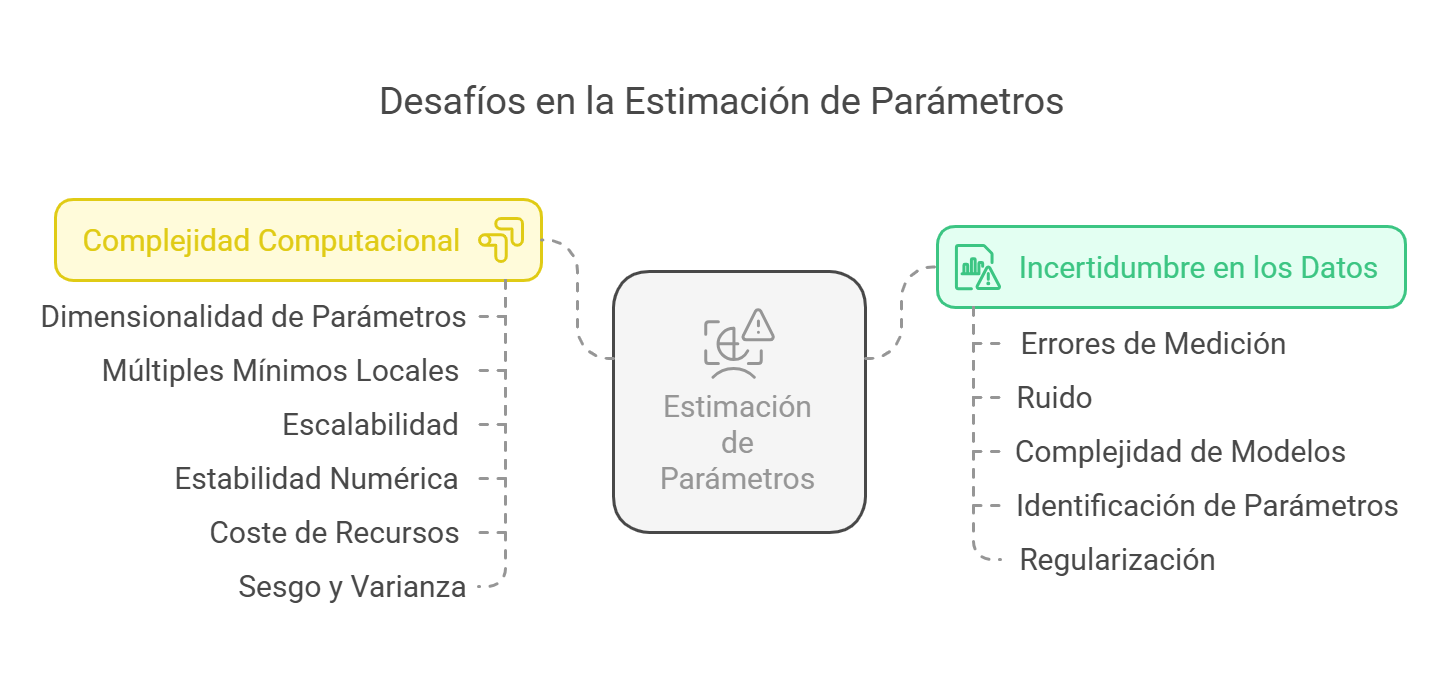
\includegraphics[width=1\textwidth]{images/visual-selection.png}
    \end{center}

        En este caso usaremos intervalos para mitigar errores en mediciones, sin embargo, presupone un desafío estimar el intervalo donde se encuentra el parámetro con un error $w(I) < \epsilon$  donde $I$ es un intervalo.\\



        \subsection*{ Problemas a resolver para conseguir una arquitectura de agentes cooperativos que integran análisis de intervalos }

        La arquitectura propuesta debe lidiar con las anteriores dificultades, los agentes deben ser capaces de actuar en un ambiente dinámico y estimar el intervalo de salida más efectivo, a su vez deben activarse ante los estímulos correctos y saber ignorar otros que ocurren en el ambiente. Los agentes deben ser capaces de cooperar entre sí y saber cuándo parar de iterar entre ellos para devolver el resultado que minimice el valor esperado. A continuación, se listan varios puntos que detallan los desafíos de la arquitectura.\\
        \begin{itemize}

            \item Modificar el espacio de llegada de cada agente para conseguir un espacio de salida
            \item Saber cómo parar dado que los agentes pueden crear ciclos de iteración entre ellos.
            \item Cada agente debe saber en cada iteración con qué agentes interactuar.
            \item Los agentes deben saber qué hacer cuando cometen errores, es decir, el error debe minimizarse en el tiempo.\\

        \end{itemize}

\label{sec:15}

    \subsection*{ Análisis de restricciones de la arquitectura de agentes}

        Para atacar el primer punto que se encuentra en las dificultades de la arquitectura en el capítulo anterior se tiene que definir el espacio de llegada que recibe el agente y el espacio de salida. Para ellos se hacen las siguientes consideraciones.\\

        Cada agente en cada iteración tiene un conjunto de precondiciones que lo activan, es decir, denotamos a $P$ como el conjunto de precondiciones y se define como $P=[ p_0,p_1,...,p_n]$ donde $p_i$ es una precondición que puede ser verdadera o falsa. $P \iff p_0 \land p_1 \land...\land p_n$. En este caso se considera verdadera que la precondición $p_i$ adquiera un valor. Por ejemplo, si el universo de precondiciones es $U=[p_0,p_1,...,p_n]$ y $P=[p_0,p_1,...,p_k]$ siendo $k<n$ entonces las precondiciones $[p_{K+1},...,p_n]$ son falsas para el agente. \\

        Se define el conjunto de acciones que puede tomar el agente donde cada acción puede ser refinada a un conjunto potencialmente infinito de acciones. Es decir, sea $F(P,X)=Z$, entonces $Z$ es una acción a tomar por el agente, donde $P$ son las precondiciones y $X$ los valores de entrada del agente \\

        En el segundo punto se requiere que los agentes deben saber parar las iteraciones puesto que pueden darse ciclos, se toman cotas superiores de iteración. Si los agentes no paran llegado este número, se devuelve el resultado generado hasta ese momento. Este método es robusto para detener las iteraciones, más adelante se verá un método iterativo que asegura la convergencia de las iteraciones. \\

        Para atacar el punto tres es necesario modelar la red de arcos entre agentes. Sea $M$ el número de agentes, si dos agentes $A$ y $B$ están conectados, entonces ocurren una de las siguientes condiciones:

        \begin{itemize}
            \item $A\rightarrow B$, $A$ 'escucha' de $B$
            \item  $B \rightarrow A$, $B$ 'escucha' de $A$
        \end{itemize}

        Si $A$ escucha de $P^n=[A_0^n,A_1^n,...,A_k^n]$ entonces las precondiciones de $A$ son $P=\lceil p_0 - \frac{1}{2} \rceil \lor \lceil p_1 - \frac{1}{2} \rceil \lor \dots \lor \lceil p_n - \frac{1}{2} \rceil$ donde: 
        $p_i=A_k$. Las expresiones $A_0^n,A_1^n,A_k^n$ se refieren al valor de las ponderaciones de los arcos $A_0,A_1,\dots,A_n$ en la iteración $k$. Es preciso notar que $p_i \in [0,1]$ \\

        Como última observación se dice que si en un instante $k$ no hay arcos entre agentes, entonces hemos convergido a un resultado final.

    \subsection*{Arquitectura de Agentes Cooperativos}

        Antes de saltar sobre los detalles de la arquitectura es necesario precisar que la arquitectura propuesta se basa en una red de agentes donde cada uno tiene una funcionalidad específica y se entrena para mejorar sus resultados. Notar que este entrenamiento es supervisado. \\

        La arquitecta está divida en cuatro agentes: los agentes de entrada, los agentes de salida, agente coordinador de acciones y el agente corrector de acciones. Lo siguiente asume que la función tiene la forma $R^n \xrightarrow{f} R^m$. \\

        Agentes de entrada: Estos agentes reciben una entrada $X$ y devuelve un valor $y$, es decir sea $FoT$ la función del agente $i$, entonces el agente recibe $(P,X)$ donde $P$ son las precondiciones, $X$ los valores de entrada y
        $T(P,X)=p_0x_0 + p_1x_1 +...+p_nx_n$ siendo $n$ el número de agentes, luego envía su resultado al puerto de salida para que otro agente la escuche. Estos agentes no son los responsables al menos de forma directa de la salida de la red.\\

        Agentes de salida: Existe un agente de salida por cada parámetro de salida estos agentes son los responsables de escuchar de los agentes de entrada y devolver la salida.
        Un punto importante es que existen tantos agentes de salida como parámetros de salida se definen. Al igual que los agentes de entrada estos implementan una función $FoT$ 
        que recibe la tupla $(P,X)$ y devuelve un valor $Y$ que es donde se espera que este la respuesta. Estos agentes se determinan al inicio del entrenamiento.

        Un punto importante a destacar es que la función de $F$ de ambos agentes, es su función característica, es decir, una función que solo implementan ellos y además se exige que sea inversible.

        Agente coordinador: Este agente se encarga de resolver en cada $k$-iteración las arcos entre agentes. Este agente recibe como entrada, la entrada a la red 
        y devuelve los arcos entre agentes. Si este agente no define arcos entre agentes, el resultado de la red está en el valor de los agentes de salida definidos. Este agente se entrena 
        a partir de los errores cometidos por sus arcos estimados. Este agente puede ser un regresor que sea capaz de recibir una entrada $m$ de parámetros y devolver
         un vector $V$ donde $|V|=(|$ Agentes de Entrada $| + |$ Agente de salida $|)(|$ Agentes de Entrada $| + |$ Agente de salida $| - 1)$ y además $v_i \in [0,1]$.
          El vector $V$ codifica la matriz $W$ de agentes donde la componente $w_{ij}$ refleja el peso de los arco entre el agente $i$ y el agente $j$, este valor es una 
          medida de cuando influye en el agente $i$ las decisiones del agente $j$.\\

        \textbf{Definición de generación}: Dada una lista $L$ de pares $(x,y)$ se define como generación al $g$-ésimo par $(x,y)$. \\

        Por cada generación la red interactúa para dado un vector $X$, devuelva un vector $Y$.\\

        Uso de intervalos \hyperref[sec:24][14]: Se usan intervalos para computar el rango de valores más probables en cada interacción de los agentes. Como hemos dicho anteriormente, cada agente recibe una combinación lineal
        que corresponde a la salida de agentes a los que está conectado, es decir $X=[X_0,X_1,...,X_n]$ donde cada $X_i$ es un intervalo. \\

        Regla de la ecuación lineal \hyperref[sec:25][15]:

                $$\frac{\left\langle \sum_{i=1}^{n} a_i x_i = b ; \; x_1 \in D_1, \ldots, x_n \in D_n \right\rangle}
                {\left\langle \sum_{i=1}^{n} a_i x_i = b ; \; x_1 \in D'_1, \ldots, x_n \in D'_n \right\rangle}$$

            dónde $i \neq j$

            \[ D'_i := D_i, \]

            \[ D'_j := D_j \cap \frac{b - \sum_{i \in [1..n] - \{j\}} int(a_i \cdot D_i)}{a_j}. \]

            Esta regla es aplicada a los números enteros, sin embargo, se puede extender a los números reales, dado que un resultado de la aritmética de intervalos la cual se define en reales.\\

        Agente corrector: Este agente corrige los arcos generadas por el agente coordinador y las envía al agente coordinador para que este las tome en cuenta en su próxima generación. Recibe como entrada el estado de los agentes de entrada y salida y los arcos entre estos. Este agente actúa una vez que la red pare sus iteraciones. \\

        Sea $V$ la salida del agente coordinador que codifica la matriz $W$, se calcula la diferencia entre el intervalo esperado y el intervalo de salida de los agentes de salida.
        Como se quiere que la red resuelva el problema en la menor cantidad de interacciones, comenzamos desde la iteración 1 a buscar qué arcos habrían dado la
        respuesta correcta. Por cada agente de salida buscamos qué o cuales agentes de entrada darian la respuesta correcta.  \\

        Se propone encontrar un grafo $G$ tal que $\underset{G}{\min}(||F(X)-Y||)$. Como se conoce la respuesta correcta $Y$, entonces la componente $y_i \in Y$ debería ser el valor de salida del agente de salida $i$-ésimo, para determinar cuáles debieron ser los valores de entrada, hacemos $r=f^{-1}(y_i)$ y $r'=T(X,P)=p_0X_0 + p_1X_1 +...+p_kX_k$ como se conocen los valores de $X$ y de $P$
        entonces el agente corrector debe buscar en la red qué agentes minimizarían $T=[|r-r'|,|r-r'|]$. Tenemos entonces dos posibles casos: \\

        Caso 1: $[|r-r'|,|r-r'|] > \sum_{i=k+1}^{n} a_iX_i$ siendo $a_i=1$, $n$ el número de agentes de salida más agentes de entrada y el intervalo de $[k+1,n]$ los agentes
        que no forman parte de la salida. Aquí basta con conectar de forma sucesiva los agentes $X_{k+j}$ con $j=1,2,..n$ hasta que $[|r-r'|,|r-r'|] \leqslant \sum_{i=k+1}^{k+j} a_iX_i$ si la relación es de igualdad, hemos encontrado los arcos,
         si es menor estricto, nos lleva al caso 2.\\

        Caso 2: Si $[|r-r'|,|r-r'|] \leqslant \sum_{i=k+1}^{k+j} a_iX_i$ siendo $a_i=1$, entonces solo despejamos uno de los agentes para encontrar el peso que iguala la ecuación
        es decir: $D(a_{k+j}) \cap \frac{[|r-r'|,|r-r'|] - \sum_{k+1}^{k+j-1} X_i}{|X_{k+j}|}$.\\

        Una vez concluidos los hallazgos en la primera iteración, esta es enviada al agente coordinador, para que se ajuste dada la tupla $(X,Y)$ siendo
        $X$ los valores de entrada a la red y $Y$ los arcos de salida, concluido esto, el agente corrector pasa a la iteración 2 y comienza nuevamente la búsqueda de el arco ideal. Una vez concluido este proceso
        el agente corrector hace el mismo proceso, pero esta vez asumiendo que la salida de la primera interacción es la entrada de la segunda iteración, es decir $\underset{X}{\min}([|r-r'|,|r-r'|])$ donde $X$ es el vector estado de la red luego de minimizar $[|r-r'|,|r-r'|]$.
        De igual forma la red continua con la siguiente iteración hasta terminar con la cola de iteraciones de la generación. Luego de pasar por todo este proceso la red comienza nuevamente con la siguiente generación de datos. \\

        Se itera dos veces sobre la pila de iteraciones porque es necesario entrenar el agente coordinador y para ello se requiere la mayor cantidad de datos posibles. Pues el primer entrenamiento se hace para rectificar los arcos erróneos, y el siguiente para aprender la respuesta correcta.
        Es importante destacar que existen infinitos grafos correctos, es por esto que el agente coordinador tiene tal comportamiento greedy.

        \subsection*{Ciclos de iteración}

         Al inicializarse la red, esta recibe un vector de entrada, luego el agente coordinador determina los agentes de salida y los arcos entre agentes. Notar que todos los agentes excepto los agentes que se determinan que son entrada, son de salida, es decir, todos los agentes de entrada reciben el vector de entrada en el primer ciclo de interacción. Para la $k$-iteración el agente coordinador cambia las arcos de los agentes y el agente $i$-ésimo recibe ahora los valores de salida de sus nuevos arcos en la $(k-1)$ iteración. Los agentes de entrada y salida comienzan a iterar hasta detenerse o hasta llegar a una cota máxima de interactividad, terminado este paso, el agente corrector corrige los arcos basado en el error cometido por la red y las envía al agente coordinador, terminado esto, estamos listo para pasar con la siguiente iteración. \\

        Notar que estos agentes paran las iteraciones si y solo si no se activa ninguna precondición de los agentes que esto a su vez conicide con que no existan arcos entre agentes. En la siguiente figura 1 se ilustra el proceso descrito: \\


        \begin{center}
                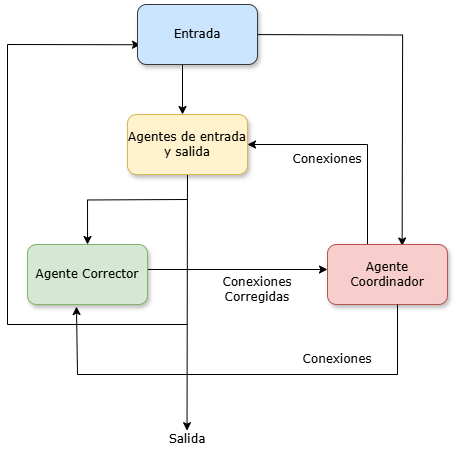
\includegraphics[width=0.6\textwidth]{images/AgentArchitecture.drawio.png}
                \begin{center}
                    fig.1 Flujo de trabajo entre los agentes
                \end{center}
        \end{center}
\chapter{Desarrollo del Algoritmo}\label{chapter:implementation}

\label{sec:16}
\subsection*{ \Large Desarrollo del Algoritmo }

 En esta sección se desarrollará el pseudocódigo del algoritmo y se analizará la convergencia y complejidad del mismo. En el siguiente gráfico se muestra el desarrollo.

 %-------------------------------
 % Main Process Algorithm
 %-------------------------------
 \begin{algorithm}[H]
 \caption{Main Process}
 \KwData{Dataset}
 \KwResult{results}
 
 \textbf{// Initialize Agents}\\
 agents.input $\leftarrow$ InitializeInputAgents()\;
 agents.output $\leftarrow$ InitializeOutputAgents()\;
 Coordinator $\leftarrow$ InitializeCoordinatorAgent()\;
 Corrector $\leftarrow$ InitializeCorrectorAgent()\;
 MaxIterations $\leftarrow$ K\;
 ConvergenceThreshold $\leftarrow$ 0.01\;
 
 \ForEach{$(X,Y)$ in Dataset}{
     InitializeInputAgentsWithX$(X)$\;
     iteration $\leftarrow$ 1\;
     converged $\leftarrow$ False\;
     stack\_edges $\leftarrow$ [ ]\;
     
     \While{iteration $\le$ MaxIterations \textbf{and} not converged}{
         \textbf{// Step 1: Coordinator determines arcs}\\
         adjacency\_matrix $\leftarrow$ Coordinator.generate\_arcs$(X)$\;
         stack\_edges.append$\bigl((\text{adjacency\_matrix},\, \text{agents.input}, \text{agents.output})\bigr)$\;
         
         \textbf{// Step 2: Check termination condition}\\
         \If{no\_arcs\_exist(adjacency\_matrix)}{
             converged $\leftarrow$ True\;
             \textbf{break}\;
         }
         
         \textbf{// Step 3: Agent computation phase}\\
         \ForEach{agent in agents}{
             agent.preconditions $\leftarrow$ calculate\_preconditions$(agent,\, \text{adjacency\_matrix})$\;
             \If{check\_activation\_conditions(agent.preconditions)}{
                 agent.output $\leftarrow$ agent.FoG(agent.preconditions, agent.inputs)\;
             }
         }
         
         delta $\leftarrow$ calculate\_max\_difference(target\_outputs, current\_outputs)\;
         \If{delta $<$ ConvergenceThreshold}{
             converged $\leftarrow$ True\;
             \textbf{break}\;
         }
         
         
         agent.inputs $\leftarrow$ agent.output\;
         
         iteration $\leftarrow$ iteration + 1\;
     }
     
         \Return AuxiliarProcess(agents, converged, adjacency\_matrix, arc\_adjustments)\;
         }
         
        \end{algorithm}

\begin{algorithm}[H]
\caption{AuxiliarProcess}
 \KwData{agents, converged, adjacency\_matrix, arc\_adjustments}
 \KwResult{results}
 
     results $\leftarrow$ CollectOutputs(agents.output)\;
     
     \If{not converged}{
        arc\_adjustments $\leftarrow$ CorrectionPhase(agents , adjacency\_matrix);
        Coordinator.update(arc\_adjustments)\;
        
        }
        \textbf{// Final output collection}
        \Return results\;

\end{algorithm}
 
 
 %-------------------------------
 % Helper Functions
 %-------------------------------

\begin{algorithm}[H]
        \caption{CorrectionPhase}
        \KwIn{agents , adjacency\_matrix}
        \KwOut{arc\_adjustments}
     \textbf{// Step 5: Correction phase}\\
         arc\_adjustments $\leftarrow$ [ ]\;
         \ForEach{iteration}{
             adjacency\_matrix, input\_agent , output\_agents  $\leftarrow$ stack\_edges[start]\;
             error $\leftarrow$ calculate\_error(output\_agents.values, Y)\;
             arc\_adjustments.append( Corrector.adjust\_arcs(error, adjacency\_matrix,agents))\;
         }
         
         
         agents.input.reset\_default\_outputs()\;
         agents.ouput.reset\_default\_inputs()\;
         
         start $\leftarrow$ 0\;
         \While{start $\le$ iteration}{
             \textbf{// Step 1: Coordinator determines arcs}\\
             adjacency\_matrix, input\_agent , output\_agents  $\leftarrow$ stack\_edges[start]\;
             
             \textbf{// Step 3: Agent computation phase}\\
             
             error $\leftarrow$ calculate\_error(output\_agents.values, Y)\;
             arc\_adjustments.append( Corrector.adjust\_arcs(error, adjacency\_matrix, agents))\;
               agents.input $\leftarrow$ agents.output
             
             start $\leftarrow$ start + 1\;
             }
         \Return arc\_adjustments\;
         
         
    \end{algorithm}
 
 \begin{algorithm}[H]
 \caption{calculate\_preconditions}
 \KwIn{agent, adjacency\_matrix}
 \KwOut{preconditions}
 preconditions $\leftarrow$ [ ]\;
 \ForEach{connected\_agent in get\_connected\_agents(agent, adjacency\_matrix)}{
     prev\_val $\leftarrow$ connected\_agent.previous\_output\;
     curr\_val $\leftarrow$ connected\_agent.current\_output\;
     max\_val $\leftarrow \max\bigl(|\text{prev\_val}|,\, |\text{curr\_val}|\bigr) + 1\times10^{-6}$\;
     precondition $\leftarrow \displaystyle \frac{|\text{prev\_val} - \text{curr\_val}|}{\text{max\_val}}$\;
     preconditions.append(precondition)\;
 }
 \Return preconditions\;
 \end{algorithm} \\
 
 \begin{algorithm}[H]
 \caption{check\_activation\_conditions}
 \KwIn{preconditions}
 \KwOut{Boolean}
 \Return all\bigl($p \geq$ ActivationThreshold for each $p$ in preconditions\bigr)\;
 \end{algorithm} \\
 
 \begin{algorithm}[H]
 \caption{CollectOutputs}
 \KwIn{OutputAgents}
 \KwOut{List of outputs}
 \Return [agent.output for each agent in OutputAgents]\;
 \end{algorithm} \\
 
 %-------------------------------
 % Corrector Agent Operations
 %-------------------------------
 \begin{algorithm}[H]
 \caption{Corrector.adjust\_arcs}
 \KwIn{error, adjacency\_matrix, agents.output, agents.input}
 \KwOut{New adjacency\_matrix}
 adjustments $\leftarrow$ []\;
 \ForEach{i,output\_agent in agents.output}{
     target $\leftarrow$ output\_agent.F$^{-1}(Y_i)$\;
     current $\leftarrow$ output\_agent.G(output\_agent.inputs)\;
     residual $\leftarrow \; |\text{target} - \text{current}|$\;
     connected\_agents $\leftarrow$ sort\_by\_relevance(agents.input)\;
     cumulative\_effect $\leftarrow$ 0\;
     updated\_weight $\leftarrow$ false\;
     cumulative\_effect $\leftarrow$ 0\;
     \ForEach{agent in connected\_agents}{
         cumulative\_effect $\leftarrow$ cumulative\_effect + agent.output\;
         adjustments.append$\bigl((\text{output\_agent},\, \text{agent})\bigr)$\;
         \If{cumulative\_effect $\geq$ residual}{
             \If{cumulative\_effect == residual}{
                 \textbf{break}\;
             }
             updated\_weight $\leftarrow$ true
             remaining $\leftarrow$ residual $-$ cumulative\_effect\;
             adjusted\_weight $\leftarrow$ remaining / last\_agent.output\;
             adjustments.append$\bigl((\text{last\_agent},\, \text{adjusted * last\_agent.output})\bigr)$\;
             update\_connection\_weight( adjustments)\;
             \textbf{break}\;
         }
     }
     \If{ not updated\_weight}{
        update\_connection\_weight(adjustments)
     }
 }
 \Return generate\_new\_adjacency\_matrix(adjustments)\;
 \end{algorithm} \\
 
 %-------------------------------
 % Coordinator Agent Operations
 %-------------------------------
 \begin{algorithm}[H]
 \caption{Coordinator.generate\_arcs}
 \KwIn{X}
 \KwOut{adjacency\_matrix}
 \Return ML\_model.predict$(X)$\;
 \end{algorithm}
 
 \begin{algorithm}[H]
 \caption{Coordinator.update}
 \KwIn{adjustments}
 training\_data.add(adjustments)\;
 retrain\_model()\;
 \end{algorithm} \\

\newpage

%%%%%%%%%%%%%%%%%%%%%%%%%%%%%%%%%%%%%%%%%%%%%%%%%%%%%%%%%%%%%%%%%%%%%%%%%%%%%%%%%%%%%%%%%%%%%

 \section*{Análisis de convergencia}
 
    El analisis de convergencia esta pricipalemnte relacionado a los agentes corrector y coordinador, puestos que estos agentes son los que guian a los agentes 
    de entrada y salida. El agente coordinador siempre encuentra una solución correcta dada la entrada y salida de la red de las infinitas posibles, por tanto se 
    puede decir que este agente converge a la ¨solución correcta¨. En los siguiente se asume que el agente coordinador converge al mínimo global: \\

    El problema de encontrar $F:X \rightarrow Y$ se ha reducido $\underset{G}{\min}(|F(X)-Y|) \leq \epsilon$ donde $G$ es un grafo en el que sus vértices son los agentes de entrada y salida. Si 
    este el agente corrector converge a $G$  entonces la red converge a $Y$ dado $X$.


 \section*{Análisis de complejidad}

    A continuación se analisa la complejidad de cada componente del sistema y luego se sintetiza para conseguir la complejidad total. \\

    Los agentes de entrada y salida tienen complejidad $N \geq O(FoG) $ siendo $N$ el número de estos agentes el agente en cuestión, esta consideración 
    sobre los agentes de entrada y salida no se puede extender dado que dichos agentes son cualquier función que de una entrada y devuelva una salida, la 
    razón principal de la cota inferior es porqque $G$ se computa en $O(N)$. El agente corrector tiene complejidad lineal con respecto al número de agentes 
    de entrada y salida, es decir $O(N)$. Sea $f$ el agente coordinador entonces este tiene complejidad $O(f)$, puesto que este es un regresor genérico. 
    El algoritmo en su totalidad tiene complejidad: 
    \begin{center}
        
        \begin{equation*}
                
                |D|(C( \max(O(F o G )) + O(f) + O(N)) + O(N)) \\
                = O(|D|C( \max(O(F o G )) + O(f) + O(N)))\\

        \end{equation*}

    \end{center}

Siendo $|D|$ el núumero de pares en el dataset y $C$ la cota máxima de iteración entre agentes.
\include{MainMatter/Resultados y Validación}

\backmatter

\begin{conclusions}
    Conclusiones
\end{conclusions}

\label{sec:19}
    \begin{itemize}
        \item  Reflexiones sobre los hallazgos y limitaciones del estudio
        \item  Implicaciones prácticas para la epidemiología computacional y el modelado matemático
       \item  Resumen de los principales aportes de la tesis
        \item  Respuestas a las preguntas planteadas al inicio sobre efectividad y convergencia.
    \end{itemize}
\textbf{ \Huge Recomendaciones} \\
    
    Si bien la propuesta es innovadora es también mejorable, en la implementación ofrecida existen múltiples limitantes que van desde el control por desbordamiento 
    de decimales y enteros hasta la falta de paralelización de los agentes y apropiada elección del agente coordinador. Entre las propuestas abiertas para el desarrollo 
    futuro está, implementar métodos más eficientes de corrección de errores para funciones no definidas en intervalos, y asi minimizar el impacto que tenga este tipo de 
    hechos en los restantes agentes para asegurar un aprendizaje estable y con poca varianza en los datos de entrada y salida. También se recomienda mejorar el control sobre 
    las restricciones definidas que debe cumplir una grafo generado por el agente coordinador.


\printbibliography[heading=bibintoc]

\label{sec:21}

\begin{itemize}

    \begin{thebibliography}

     \bibitem[1]{Ortiz2022} {Algoritmo Intervalar: Una alternativa de solución del problema de estimación de parámetros en la Interface Eagle. Autor: Rocio Ortiz Gancedo, Tutores: Dra. Aymée Marrero Severo, Lic. Daniela González Beltrán, Trabajo de Diploma presentado en opción al título de Licenciado en Ciencia de la Computación, 2022, Universidad de la Habana Facultad Matemática y Computación.}
     \label{sec:1}

    \bibitem[2]{}\href{https://doi.org/10.1038/s41598-022-06992-0}{ articule Deep learning forecasting using time varying parameters of the SIRD model for Covid 19 tipo: JOUR, autores: Bousquet, Arthur ,Conrad, William H., Sadat, Said Omer, Vardanyan, Nelli, Hong, Youngjoon, fecha: 2022/02/22, JO: Scientific Reports, SP: 3030, volúmen 12, número de la edición: 1, número estándar   - 2045-2322, DO  - 10.1038/s41598-022-06992-0, ID: Bousquet2022.}
     \label{sec:2}

    \bibitem[3]{}  \href{https://www.redalyc.org/journal/3238/323864536006/html/}{Bayesian modeling of spatio temporal patterns of the cumulative incidence of COVID-19 in municipalities of Mexico, de Gerardo Núñez Medina, \href{https://revistarelap.org/index.php/relap}{ Revista Latinoamericana de Población}, vol. 15, núm. 28, pp. 160-178, 2021, DOI:  https://doi.org/10.31406/relap2021.v15.i1.n28.6}
      \label{sec:3}

    \bibitem[4]{}\href{https://www.semanticscholar.org/paper/Contributions-to-the-mathematical-theory-of-V.-of-a-Kermack-Mckendrick/7beba9b40b692c2daa9975861394aefddcbe602b}{ Kermack WO, McKendrick AG. Contributions to the mathematical theory of epidemics: V. Analysis of experimental epidemics of mouse-typhoid; a bacterial disease conferring incomplete immunity. Journal of Hygiene. 1939;39(3):271-288. doi:10.1017/S0022172400011918}
\label{sec:4}

    \bibitem[5]{}\href{https://personal.us.es/sergio/PDocente/lectura.pdf}{El Método de Mínimos Cuadrado, Sergio A. Cruces Álvarez, UNIVERSIDAD DE SEVILLA}
     \label{sec:5}

    \bibitem[6]{}\href{https://inria.hal.science/hal-04100467}{Daniel Bernoulli, Dominique Chapelle. Essai d'une nouvelle analyse de la mortalité causée par la petite vérole, et des avantages de l'inoculation pour la prévenir. 2023.⟨hal-04100467⟩}
\label{sec:6}

    \bibitem[7] {}\href{ https://www.google.com/books/edition/Introduction_to_Interval_Analysis/kd8FmmN7sAoC?hl=en&gbpv=0 }{Introduction to Iterval Analysis, authors:
    Ramon E. Moore, Worthington, Ohio, R. Baker Kearfott, University of Louisiana at Lafayette, Lafayette, Louisiana, Michael J. Cloud, Lawrence Technological University, Southfield, Michigan, editorial: Society for Industrial and Applied Mathematics, Philadelphia,  Publisher:Cambridge University Press, Published:April 16, 2009, ISBN:9780898716696, 0898716691,

Format:Paperback}

     \label{sec:7}

    \bibitem[8] {}\href{https://www.scielosp.org/pdf/rsap/2020.v22n2/132-137/es}{Predicciones de un modelo SEIR para casos de COVID-19 en Cali, Colombia , autores Ortega-Lenis, Delia ,Arango-Londoño, David, Muñoz, Edgar, Cuartas, Daniel E., Caicedo, Diana, Mena, Jorge, Torres, Miyerlandi, Mendez, Fabian.  Revista de Salud Pública apr 2020, Volume 22 N. 2 Pages 132 - 137,  DOI:https://doi.org/10.15446/rsap.v22n2.86432  }
     \label{sec:8}

    \bibitem [9]{}Resolución del problema de la Optimizacion Global mediante Análisis de Intervalos, Gretel Domínguez Rodríguez Tutores: Dra. Aymée Marrero Severo, MSc. Jorge Barrios Ginart, Trabajo de Diploma presentado en opción del título de Licenciado en Ciencia de la Computación, junio de 2009, Universidad de la Habana Facultad Matemática y Computación
     \label{sec:9}

    \bibitem [10]{ } \href{https://lccn.loc.gov/2019047498 }{Artificial intelligence: a modern approach / Stuart J. Russell and Peter Norvig, authors: Stuart Russell and Peter Norvig ,2020, Identifiers: LCCN 2019047498 | ISBN 9780134610993 (hardcover), Subjects: LCSH: Artificial intelligence. Classification: LCC Q335.R86 2021 | DDC 006.3–dc23, LC record available at https://lccn.loc.gov/2019047498, ScoutAutomatedPrintCode, ISBN-10: 0-13-461099-7, ISBN-13: 978-0-13-461099-3, capítulos 9,10,11}
     \label{sec:10}

    \bibitem[11]{} \href{https://ia601500.us.archive.org/19/items/b28985266/b28985266.pdf}{On the Mode of Communication of Cholera, by JOHN SNOW, M.D., JIEMBEH OF THE ROYAL COl.LEGE OF PHYSICIANS, FELLOW OF THE ROYAL MED. AND CHIR. SOCIETY, FELLOW AND VICE- PRESIDENT OF THE MEDICAL SOCIETY OF LONDON. Second Edition, LONDON JOHN CHURCHILL, NEW BURLINGTON STREET. }
     \label{sec:11}

    \bibitem[12]{}  \href{https://www.nature.com/articles/s41598-022-22945-z#citeas}{ Castro, B. M., Reis, M. M. Salles, R. M. Multi-agent simulation model updating and forecasting for the evaluation of COVID-19 transmission. Scientific Reports 12, 22091 (2022) }
     \label{sec:22}

     \bibitem[13]{}  \href{ https://doi.org/10.1093/aje/kwn118}{Title: A New Tool for Epidemiology: The Usefulness of Dynamic-Agent Models in Understanding Place Effects on Health Authors: Amy H. Auchincloss, Ana V. Diez Roux Journal: American Journal of Epidemiology. Volume: 168 ,Number: 1, Pages: 1-8 2008,  May ,DOI: 10.1093/aje/kwn118}
    \label{sec:23}

    \bibitem[15]{}  \href{https://www.cambridge.org/core/books/principles-of-constraint-programming/C008FB32571F66C3EE0EEEBDE1F98A7D}{1. Apt K. Frontmatter. In: Principles of Constraint Programming. Cambridge University Press; 2003:i-iv.}
    \label{sec:24}

    \bibitem[15]{}  \href{https://www.cambridge.org/core/books/principles-of-constraint-programming/C008FB32571F66C3EE0EEEBDE1F98A7D}{1. Apt K. Frontmatter. In: Principles of Constraint Programming. Cambridge University Press; 2003:i-iv.}
    \label{sec:25}

    \bibitem[16]{}  \href{http://saber.ucv.ve/bitstream/10872/14678/1/T026800014698-0-FinalDefensa_JoseLuisRomero-000.pdf}{UNIVERSIDAD CENTRAL DE VENEZUELA FACULTAD DE AGRONOMÍA COMISIÓN DE ESTUDIOS DE POSTGRADO POSTGRADO EN ESTADÍSTICA Métodos de Máxima Verosimilitud para la Estimación de Parámetros en Diseños
    Factoriales Mixtos pxq y sus Aplicaciones en la Agroindustria  Autor: Ing. José L. Romero Tutor: Dr. Manuel Milla Consejeros: Dr. Miguel Balza Dr. Franklin Chacín}
    \label{sec:26}

    \bibitem[17]{}\href{https://cimat.repositorioinstitucional.mx/jspui/bitstream/1008/255/2/TE%20388.pdf}{Centro de Investigaci´on en Matem´aticas, A.C. Estimación de los parámetros de un modelo haciendo uso de correspondencias con incertidumbre Tesis que para obtener el grado de Maestro en Ciencias con Especialidad en Computación y Matemáticas Industriales presenta Iván Maldonado Zambrano Director de Tesis Dr.Javier Flavio Vigueras Gómez Dr. Arturo Hernández Aguirre Guanajuato, Gto. Julio de 2011}
    \label{sec:27}

    \bibitem[18]  {}\href{https://cimat.repositorioinstitucional.mx/jspui/bitstream/1008/255/2/TE%20388.pdf}{Optimización No Lineal Basada en “Enjambre de Partículas” M. Susana Moreno, Aníbal M. Blanco, Planta Piloto de Ingeniería Química PLAPIQUI (Universidad Nacional del Sur - CONICET) Camino La Carrindanga km. 7 - 8000 Bahía Blanca - Argentina {smoreno, ablanco}@plapiqui.edu.ar}
    \label{sec:28}

    \bibitem[19]  {}\href{http://www.scielo.org.bo/scielo.php?script=sci_arttext&pid=S1562-38232020000100005&lng=es&tlng=es.}{Vargas, J. C., Cruz-Carpio, Carlos Andrés. (2020). Estudio del método Monte Carlo en simulaciones para la estimación del valor de pi. Revista Boliviana de Física, 36(36), 26-32. Recuperado en 07 de febrero de 2025}
    \label{sec:28}

    \bibitem[20]{}\href{https://www.semanticscholar.org/paper/A-Bayesian-approach-to-parameter-estimation-in-HIV-Putter-Heisterkamp/5eaa80435e642203bb1333011d1143a5b90577d2?utm_source=direct_link}{Putter, H., Heisterkamp, S.H., Lange, J.M.,  Wolf, F.D. (2002). A Bayesian approach to parameter estimation in HIV dynamical models. Statistics in Medicine, 21.}
    \label{sec:30}

    \bibitem[21]{}  Revista Ingeniería y Región Vol. 24 Julio-Diciembre 2020/Universidad Surcolombiana Artículo de Investigación Variación temporal de los índices de sensibilidad de un modelo de cultivo para jitomate en invernadero Antonio Martinez Ruíz PhD martinez.antonio@inifap.gob.mx Genaro Pérez Jiménez M.C. perez.genaro@inifap.gob.mx, Cándido Mendoza-Pérez PhD mendoza.candido@colpos.mx Felipe Roberto Flores-de la Rosa PhD. flores.felipe@inifap.gob.mx Miguel Servin Palestina servin.miguel@inifap.gob.mx Fecha de recibido:18/10/2020 Fecha de revisión:27/10/2020 Fecha de aprobación:21/12/2020 DOI: 10.25054/22161325.2833
    \label{sec:31}

    \bibitem[22]{} \href{https://theses.hal.science/INRIA/hal-04798230v1}{Physics-informed neural networks for parameter estimation and simulation of a two-group epidemiological model Kawtar Idhammou Ouyoussef, Jaafar El Karkri Leon Matar Tine and Rajae Aboulaich LERMA Laboratory, Mohammadia School of Engineering Mohammed V University in Rabat, Rabat, Morocco Inria, Universite de Lyon, 69100 Villeurbanne, France Institut Camille Jordan, CNRS UMR5208 Universite Claude Bernard Lyon 1 69603 Villeurbanne, France kawtaridhammou@research.emi.ac.ma elkarkri@emi.ac.ma leon-matar.tine@univ-lyon1.fr aboulaich@emi.ac.ma Published 19 July 2024}
    \label{sec:32}

    \bibitem[23]{} \href{https://ai.stanford.edu/~nilsson/OnlinePubs-Nils/PublishedPapers/strips.pdf}{STRIPS: A New Approach to the Application of Theorem Proving to Problem Solving' Richard E. Fikes Nils J. NHsson Stanford Research Institute, Menlo Park, California Recommended by B. Raphael Presented at the 2nd IJCAI, Imperial College, London, England, September 1-3, 1971.}
    \label{sec:33}

    \bibitem[24]{} \href{https://courses.cs.washington.edu/courses/cse473/06sp/pddl.pdf}{McDermott, D., Ghallab, M., Howe, A.E., Knoblock, C.A., Ram, A., Veloso, M.M., Weld, D.S., Wilkins, D.E. (1998). PDDL-the planning domain definition language.}
    \label{sec:34}

    \bibitem[25]{} \href{https://doi.org/10.1145/321033.321034}{Martin Davis and Hilary Putnam. 1960. A Computing Procedure for Quantification Theory. J. ACM 7, 3 (July 1960), 201–215.}
    \label{sec:35}

    \bibitem[26]{} \href{https://www.sciencedirect.com/science/article/abs/pii/0004370277900078?via%3Dihub}{Mackworth, A.K. (1977). Consistency in Networks of Relations. Artif. Intell., 8, 99-118.}
    \label{sec:36}

    \bibitem[37]{} \href{https://www.swi-prolog.org/pldoc/doc/_SWI_/library/clp/clpfd.pl}{clpfd.pl -- CLP(FD): Constraint Logic Programming over Finite Domains}
    \label{sec:27}




    \end{thebibliography}

\end{itemize}

\end{document}